% !TEX encoding = UTF-8 Unicode
% !TEX program = pdflatex
% !TEX spellcheck = en_US


% In order to correctly compile this document,
% execute the following commands:
% 1. pdflatex
% 2. pdflatex
% 3. pdflatex



\documentclass[amsthm,ebook]{saparticle}

% IF YOU USE PDFLATEX
\usepackage[utf8x]{inputenc}
% if you write in english and in greek
\usepackage{ucs}
\usepackage[greek,english]{babel}
\languageattribute{greek}{polutoniko}

% IF YOU USE XELATEX
%\usepackage{polyglossia}
% if you write in italian
%\setmainlanguage{italian}
% If you want put some ancient greek:
%\setotherlanguage[variant=polytonic]{greek}
%\newfontfamily{\greekfont}[Ligatures=TeX]{Palatino Linotype}

% dummy text (remove in a normal thesis)
% remove if not necessary
\usepackage{siunitx}
%Natbib for bibliography management
\usepackage[authoryear]{natbib}
% custom commands
\newcommand{\bs}{\textbackslash}

%%%%%%%%
%TITLE:%
%%%%%%%%
\title{Latin epigraphy for the visually impaired. New technologies to favour universal accessibility}
\author[mne]{Francesca Licordari\corref{first}}
\address[mne]{Museo Nazionale Etrusco di Villa Giulia, Roma}
\cortext[first]{Corresponding author. Email: francesca.licordari@beniculturali.it}
\date{2015-11-19}
\begin{document}
\maketitle
\begin{abstract}
The problem of accessibility to works of art for the visually impaired can be extended to a system such as Latin
epigraphy, which presents great difficulties since the engraved letters are not clear to the touch. The technology of
3D printing allows the creation of materials that make it easier to read epigraphic texts in following the ``design for
all'' principle demonstrating an economic, rapid technique that is easy to implement and reasonably robust.
\end{abstract}
\keywords{Accessibility, visually impaired, 3D printing, design for all, Braille, epigraphy}




\section{Introduction}
\noindent The Declaration of the Rights of Deaf-Blind Persons, adopted by the UN in 1979, provides that every blind or deaf person
has the right to enjoy the same privileges, guaranteed to all people and to have their aspirations and abilities
recognized and respected. These principles are reaffirmed by the UN Convention on the Rights of Persons with
Disabilities of 2006, which states (Art. 30) that the Member States must recognize 

\begin{quotation}
the right of persons with disabilities to take part on an equal basis with others in cultural life and should take all appropriate measures to
ensure to persons with disabilities:

\begin{description}
\item[A] enjoy access to cultural materials in accessible formats;

\item[B] enjoy access to television programs, films, theater and other cultural activities, in accessible formats;

\item[C] enjoy access to places of cultural activities, such as theaters, museums, cinemas, libraries and tourism services,
and, as far as possible, to monuments and sites of national cultural importance.

\end{description}

\end{quotation}
The problem of accessibility and enjoyment of works of art by the visually impaired has long existed. Sculptures, which
are sometimes designed to be touched, and sometimes are permitted to be touched, provide the possibility for blind
viewers to benefit directly from the experience of the original artwork. For two-dimensional paintings this is of
course not possible. It is necessary to create three-dimensional resin reliefs. This same issue has recently been
understood to exist also in other artistic disciplines, including that of archaeology. This of course includes
epigraphy, which is the study of all those materials which have written inscriptions. Most relevant to this is Latin
Epigraphy, simply because it is the one closest to our language and which uses the same graphic signs of our own
writing.

The bibliography in this area of study is unfortunately not very comprehensive, especially as regards the epigraphic
field; but advances are even now being made. In Italy, the most important studies are conducted by the ``Museo Tattile
Statale Omero'' in Ancona, which, being a museum of statuary, is mainly engaged with reproductions and the accessibility
of tactile sculptures. The same work, involving the reproduction of paintings, is being carried out by the ``Museo
Tattile Anteros'' in Bologna. It is no coincidence that Italian studies in this field are the most important done at the
international level. This is mainly due to the fact of Italy’s great artistic and epigraphic heritage, which makes it
the country where the problem is most profoundly felt.

The results of this paper are derived primarily from field studies, and also through various assistance and support
provided in partnership with people of both limited vision and complete visual impairment who tested the strengths and
weaknesses of the materials which will be referenced in this paper.


\begin{figure}[!hbp]
\centering
 \includegraphics[width=\columnwidth]{1tactiletourVillaGiulia.JPG}
\caption{Sculptures are permitted to be touched in the National Etruscan Museum of Villa Giulia in Rome}
\label{fig:1}
\end{figure}


\begin{figure}[!hbp]
\centering
 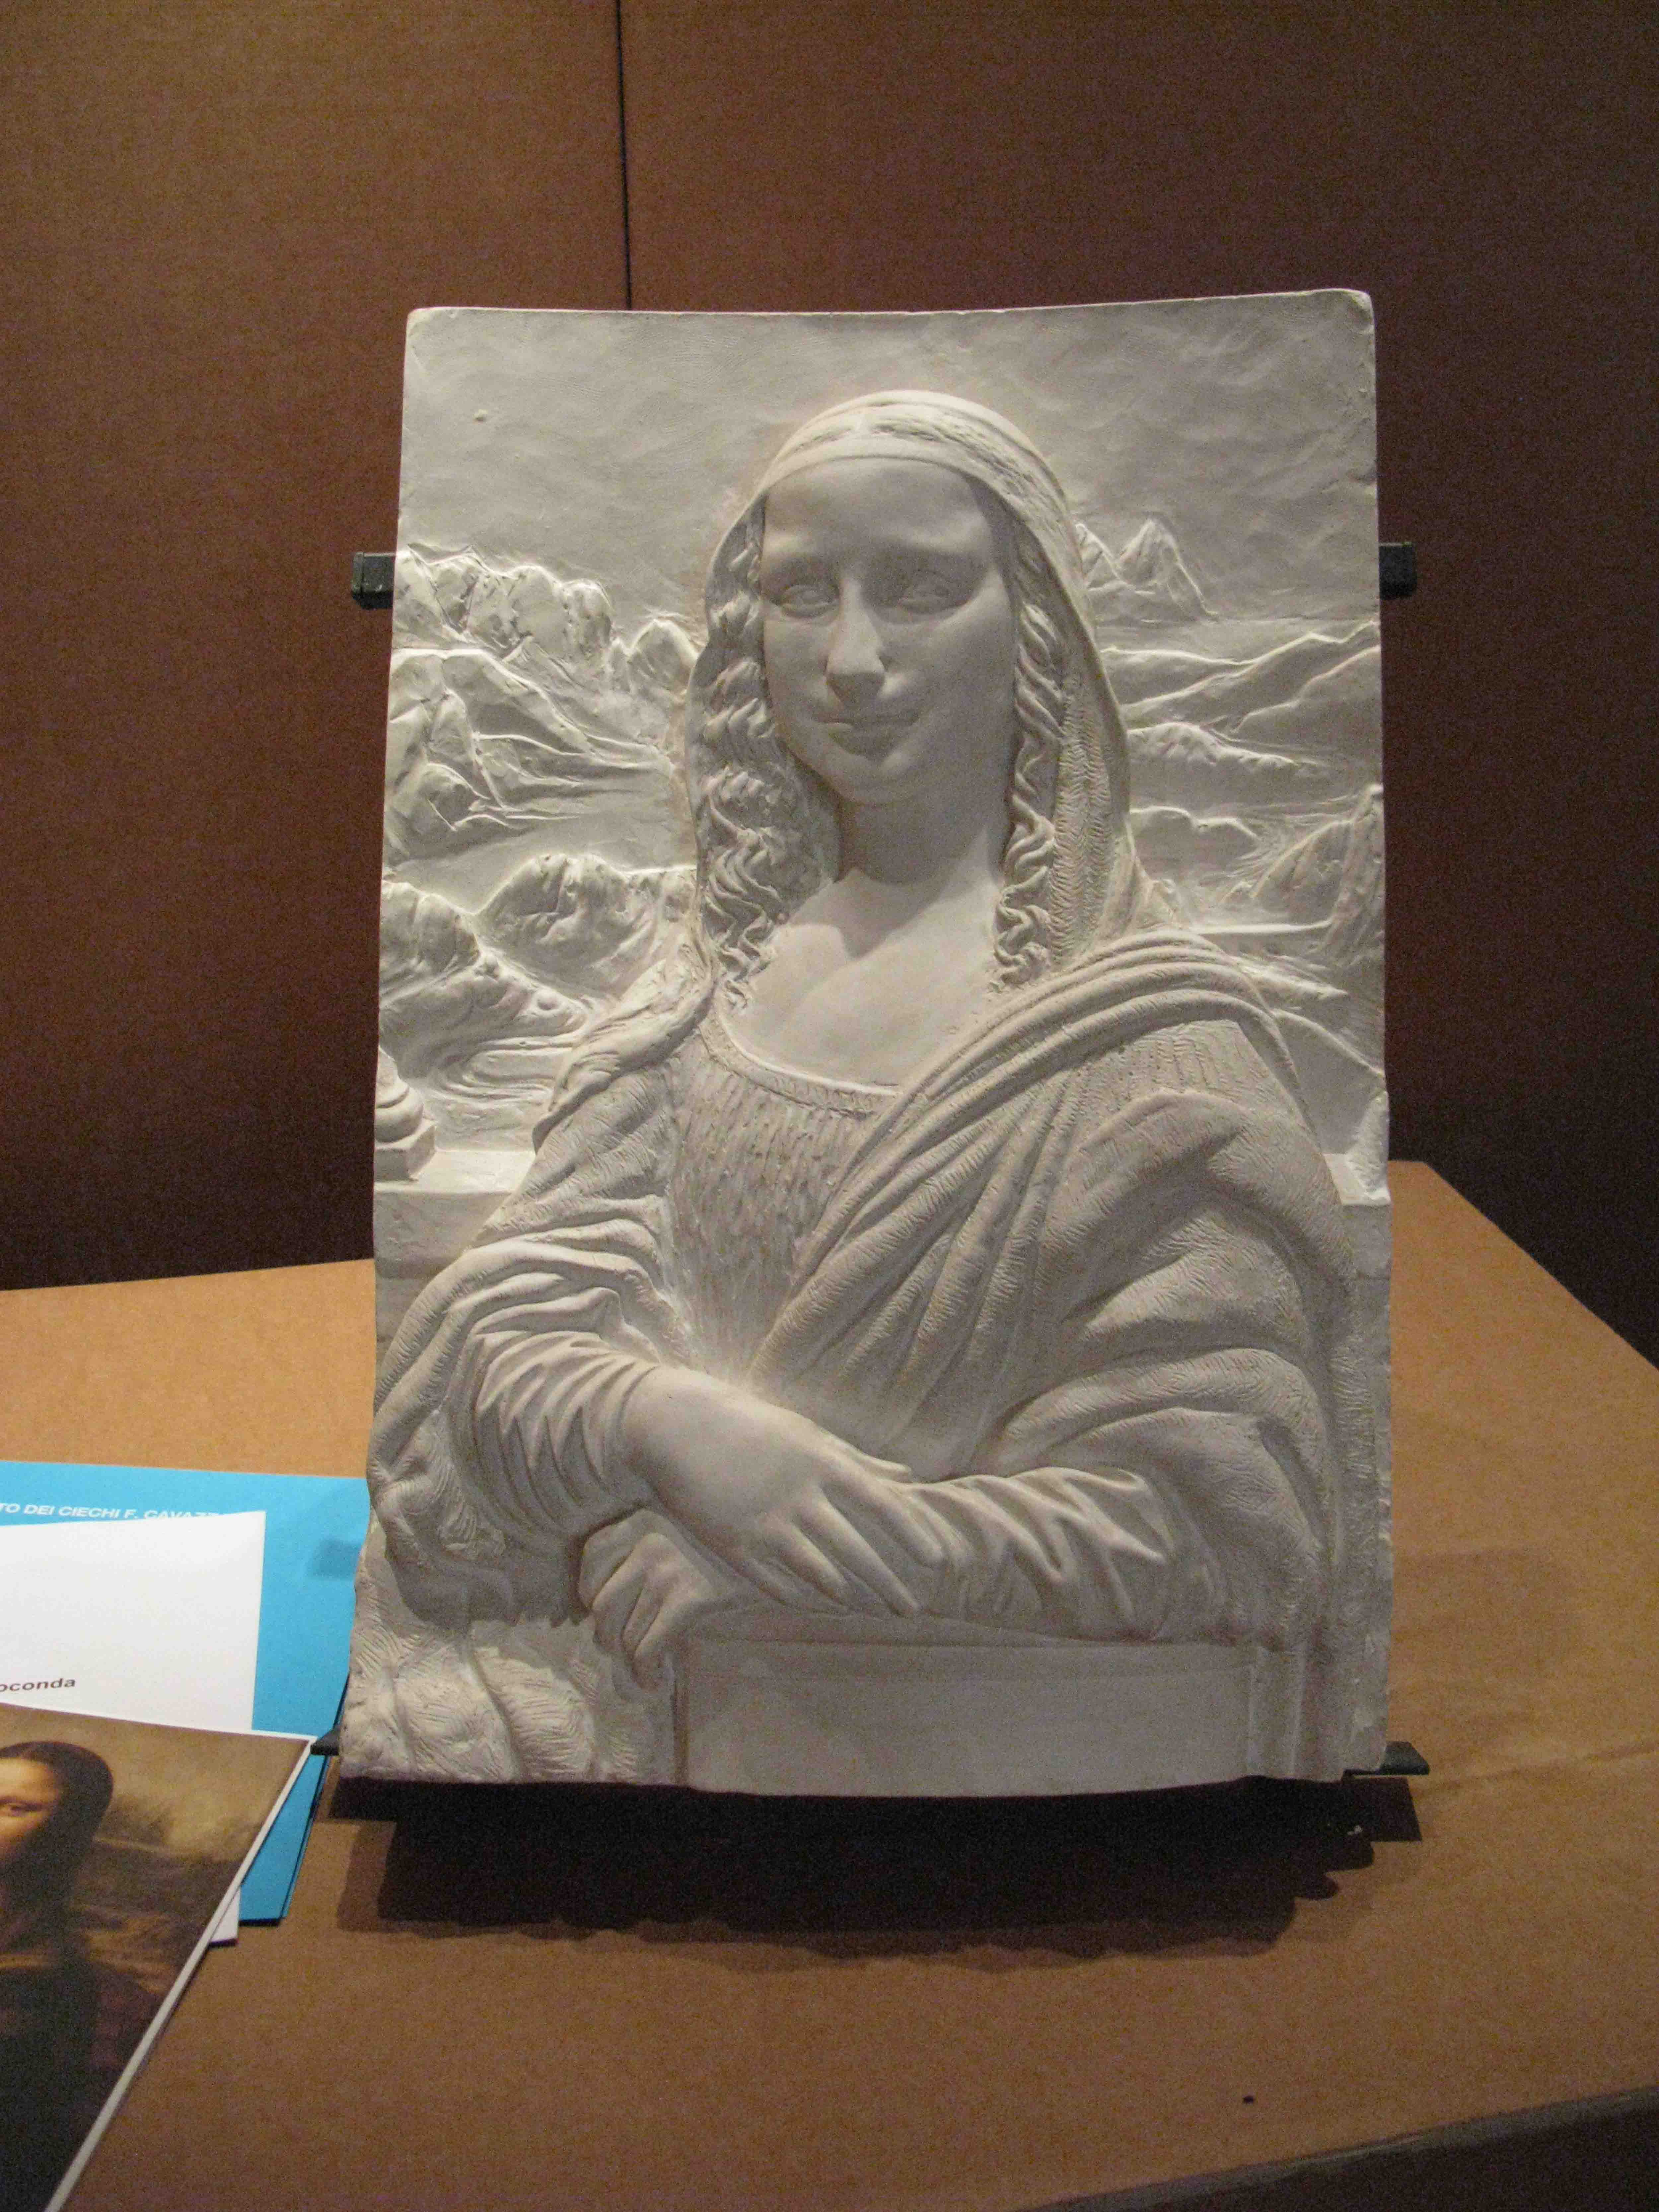
\includegraphics[width=\columnwidth]{2resinreliefMonaLisa.JPG}
\caption{Resin relief of the Anteros Museum: Mona Lisa}
\label{fig:2}
\end{figure}



\section{Problems in Understanding Epigraphy}
\noindent The field of epigraphy, always considered highly specialized, can be of great fascination to people with visual
impairment. Some may have studied ancient languages at school, especially Latin, and so feel the need to have practical
examples for the understanding of the subject; and some may be attracted out of curiosity. It is obvious that
accessibility to the inscriptions for such people involves a number of difficulties, and not just that of understanding
the texts, which are often full of abbreviations. There is, as well, a certain percentage of the blind who never
learned to read and write. Not infrequently, they may only know capitals, but not cursive characters. The inscriptions,
which appear so sharp to us that we are often tempted to touch them with our hands to follow the course of the
incisions, actually create complicated problems for the blind.

In this regard it should be noted that the sense of touch is neurologically and physiologically more suited to perceive
what is protruding from a surface, rather than to what is engraved upon it. This is a fundamental difference from the
sense of sight, which is suited to perceive contrasts in color and between light and shadow, regardless of the
technique used to create them (reliefs or incisions). The groove of a letter, even if deeply incised, is not always
easily distinguishable to the touch, while a written relief almost always is. Therefore, to allow for the visually
impaired the proper accessibility to an inscription, the original needs to be touched while, however, exploiting
resources to make transliterations in relief and Braille.

The creation of panels and captions in Braille can help in the understanding of a text, but it can not be the only
solution, as only a percentage of the blind understand Braille. A prerequisite for this is the instruction be given at
a young age, something that unfortunately does not always happen. With widespread computer usage, the majority of blind
children learn to write on the computer, which supplies speech synthesizer without the need for Braille. In this way,
the art work is losing its esthetic value.

A visually impaired person, however, has normally never learned Braille because with the right font size and adequate
lighting he can read standard writing - albeit with difficulty. In many cases, their blindness occurs in advanced age,
or as a result of illness or accident. In such situations, the writing that is understood had been taught in their
school years.

As Braille graphically occupies comparatively more written space, there are distances and dimensions that must be met
and therefore their characters cannot be made smaller as can be done with printing presses or computers. It follows,
then, that the explanations in Braille accompanying museum art works need to be more concise, in large part because
their reading needs to be done with both hands, making it uncomfortable to stand reading the texts for very long.

In the case, then, of writings on mosaics, of paintings and designs, it is not even possible to perceive the form and
the depth of the ductus. The surface appears completely flat to the touch.

The best solution to make the epigraphic media available to the visually impaired turns out to be, therefore, one that
involves more visitors who can better understand the artwork. In this regard, understood that the chance of
touching an original work wherever possible is a uniquely fascinating act, it becomes necessary to propose
reproductions that can make the material accessible by following the concept of ``design for all,'' which is adaptable to
all types of art. As rightly noted by the scholar and educator Enzo Tioli \citep{Tioli2006},
this principle can be defined as ``identical, whenever possible, equivalent when that is not possible.'' All that can be
touched and seen in the original work constitutes the ``identical'', the use of a copy constitutes the ``equivalent''.







\section{The Techniques of Accessibility}
\noindent In the world of epigraphy, casts of inscriptions are often used, both to facilitate their study by specialists,
and also to replace those exhibits that had been located outside and brought indoors to protect them from weather
conditions. These casts, if used by the visually impaired, present the same problems of accessibility as the original
in terms of the difficulty of understanding the incision’s grooves. It is necessary, therefore, to have a reproduction
of a different type, upon which the letters can be transliterated in relief.

At this time of experimentation in this direction, there are not as yet many constructed, the reason being that works of
touchable statuary without additional aids are given more importance; and masterpieces of painting in art history are
made accessible by means of a process of conversion to relief.

A remarkable attempt, albeit with many limitations, is the one created in Rome’s Capitoline Museums that, for their
epigraphic collection, the Lapidary Gallery, created in 2007 a touch accessible project, in collaboration with the NGO
Museum - Voluntary Association of Museums. Here, works with the most significant inscriptions of the largest sizes and
preferably with reliefs were selected and availed in a way as to give the visually impaired a sense of the monument as
a whole, rather than only of the text itself. The technique utilized led to a Braille book entitled Messages from
Stone, published by Silvio Zamorani, who has specialized in Braille publications. The book was created with images in
relief; but unfortunately this technique is not very perceptible to the touch and quickly becomes outdated.

The just mentioned reliefs, in fact, hardly stands out from the outline of the exhibit and we opted for the choice of
reproducing the epigraphic texts only in print with overlapping respective Braille letters. For reasons of the problems
of adequate space previously mentioned, the transliteration into Braille is not always complete nor accurate, as in the
case of the relief dedicated to Silvanus and to the Genius of the Equites Singulares. In the latter instance, the
missing transliteration of certain words was somewhat justified by the lack of space; but such a choice deprives the
blind of the total understanding of the work. The dedicatee, Marcus Ulpius Fructus, is shown in Braille without
praenomen and nomen, thereby omitting an important element of dating and contextualization. In the caption, the text in
Braille and in writing does not coincide, thereby losing the abbreviation’s clarity and the translation’s exactness.

The technical device for this publication and the panels presented in the museum gallery is that of graphic Braille
print, a special printing technique of simple and rapid implementation, capable of reproducing text and drawings using
closely spaced Braille dots. This means that sometimes the difference between the signs of writing and those of the
drawings is imperceptible to the touch. Moreover, the device was also forced to work on only one level of relief.
Having multiple levels available to distinguish the different elements of the object, is similar to that of using
different tones of different colors. It is in this way possible to recognize the design of one level and the writing of
another - the differences of only a few millimeters would be sufficient.

\begin{figure}[!hbp]
\centering
 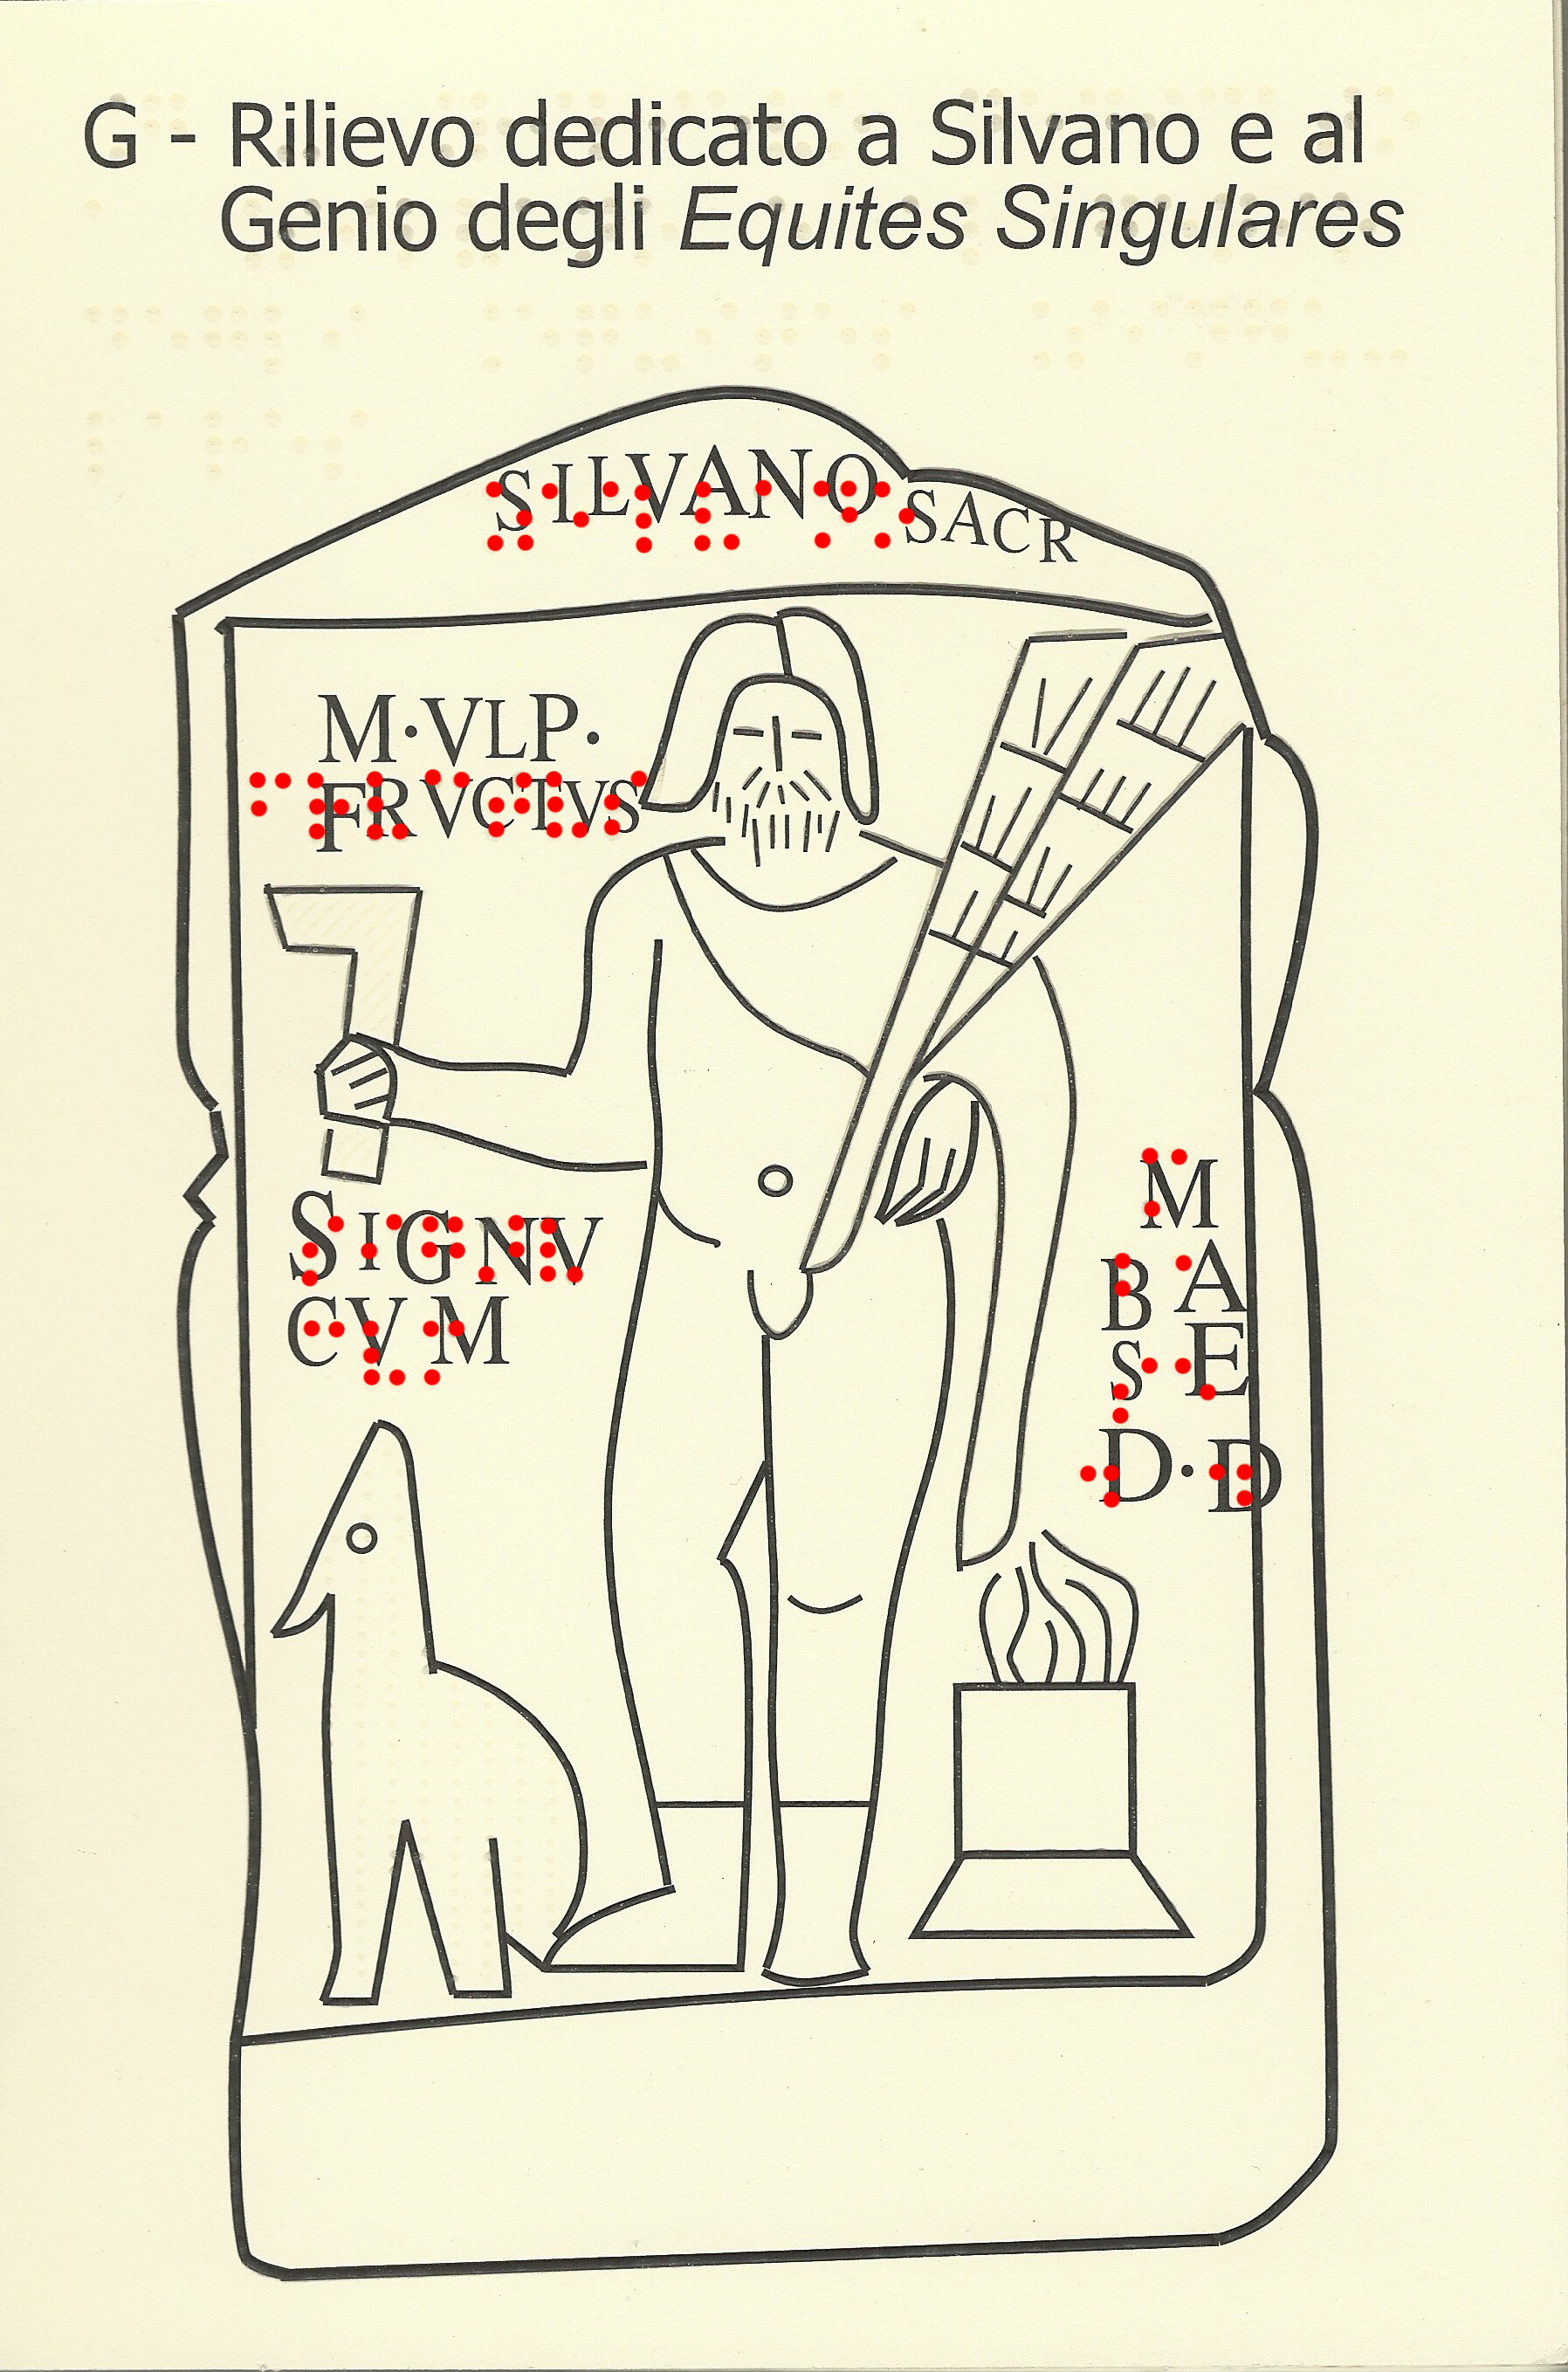
\includegraphics[width=\columnwidth]{3graphicprintBrailleMarcusUlpiusFructus.jpg}
\caption{The technical device of graphic Braille print for the panel of Marcus Ulpius Fructus}
\label{fig:3}
\end{figure}


A technique which solves this problem is that of the Thermoform, that is a relief obtained from a plastic material,
formed in a metal matrix. This type of technique is the one most used for the creation of teaching aids in schools for
the blind (in this regard see \url{www.prociechi.it}). But the technique proves to be very expensive in the creation of the
original matrix, as well as for the reproductions of individual pieces. The costs come down significantly when multiple
copies are derived. The ease of obtaining new copies compensates for the rapid deterioration of the material.

\begin{figure}[!hbp]
\centering
 \includegraphics[width=\columnwidth]{4thermoform.JPG}
\caption{The technique of the Thermoform with caption in Braille}
\label{fig:4}
\end{figure}


An additional system of reproduction, which is still in use but is gradually disappearing, is the Minolta Heater with
printing granules. This enables the quick printing of designs and writing on a paper little thicker than that of normal
stationary. It has never been used in reproduction of inscriptions for the blind and there would be nothing that could
prevent that. But based on experiences and tests made by people with visual disabilities, it can be said that the
resulting relief is not very pronounced to the touch, to this should be added the poor resistance of the characters,
which often, after prolonged use, tend to become damaged or completely lost. The Minolta system is therefore a still
utilizable technique useful in creating images for brief exposure, but it must be avoided for reproductions intended
for permanent collections.



\begin{figure}[!hbp]
\centering
 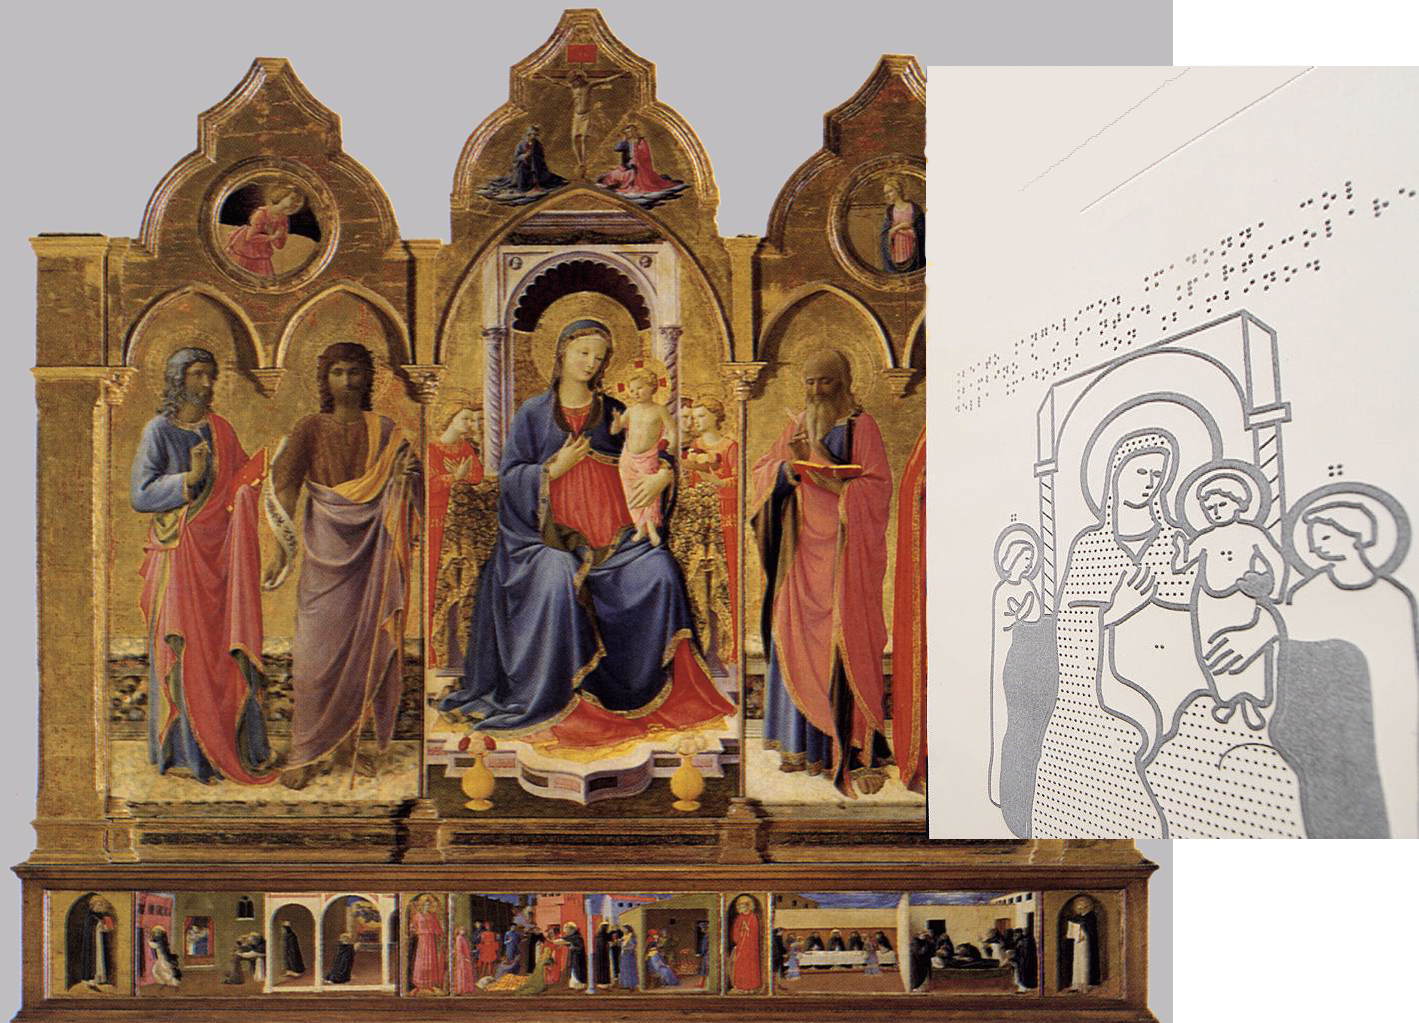
\includegraphics[width=\columnwidth]{5Minoltaheather.jpg}
\caption{Reproduction with printing granules (Minolta Heather) of the Cortona Triptych by Fra Angelico}
\label{fig:5}
\end{figure}



\section{3D Printing}
\noindent The new frontier in the understanding of works of art for the sight impaired is provided by 3D printing, which proves to
be both economical, fast, easy to implement, and durable. It is a single technique, which gathers together the
advantages of the techniques already highlighted and overcomes the defects of poor durability. Moreover, as the name
implies, it allows the introduction of the third dimension, which until now had never been possible, allowing the blind
person to be able to better perceive objects in space. This problem maybe not obvious in the case of inscriptions on
plates, but presents itself when we deal with sculptured monuments containing inscriptions.

Precisely from this technology in 2007, coordinated by Prof. Massimo Bergamasco and the Perceptual Robotics Laboratory
(Percro), was developed the project PURE-FORM, which led to the creation of a virtual museum, which gives visitors the
chance to see and ``touch'' objects, in particular digital sculptures, belonging to different historical periods and from
different contexts. All of this is based on a digital scan of the artworks stored in a database, thus offering a wide
choice, and reproduced on a touch screen display. In this project the focus was also placed exclusively on sculptures,
which already possess the third dimension, while the epigraphic content has been completely omitted. The creation of a
display, in practice a computer, allows on the one hand more accessibility to artworks, but on the other deprives the
user of the opportunity to travel to a place where they could personally experience the work’s features. It must not be
forgotten that a museum or an archaeological site are not just warehouses and storage sites.

The great advantage of 3D printing is that it materially allows more types of reproduction fundamental to human
comprehension that can be joined together and be touched and perceived as if real:

\begin{itemize}
\item Original

\item Original with fractures and abrasions and signs of aging

\item Integrated original

\item Reproduction with transliterated reliefs

\item Reproduction of the original with Braille overlay.
\end{itemize}


A copy could be thought of in its original 1:1 scale, that can be regularly handled to give an idea of its dimensions;
to another with letters in relief, rather than etched, for a better understanding of the texts; the realization of
individual fragments of inscriptions that could then be put together like a puzzle, just as the epigraphist does. Very
often, in fact, the inscription is the result of a recombination of the fragments. Moreover the inscription may be
created, by modeling it in a different way to the touch where the integration between the fragments is clear. In this
way the visually impaired would be able to approach epigraphy in almost the same way as any sighted person. This is
notwithstanding the need for explanatory captions accompanied by transliteration and the noting of the abbreviations,
which of course may not be clear to the layman.


\begin{figure}[!hbp]
\centering
 \includegraphics[width=\columnwidth]{6smallmodel3Dprinting.JPG}
\caption{Small model in 3D printing of the Sarcophagus of the Spouses}
\label{fig:6}
\end{figure}

\begin{figure}[!hbp]
\centering
 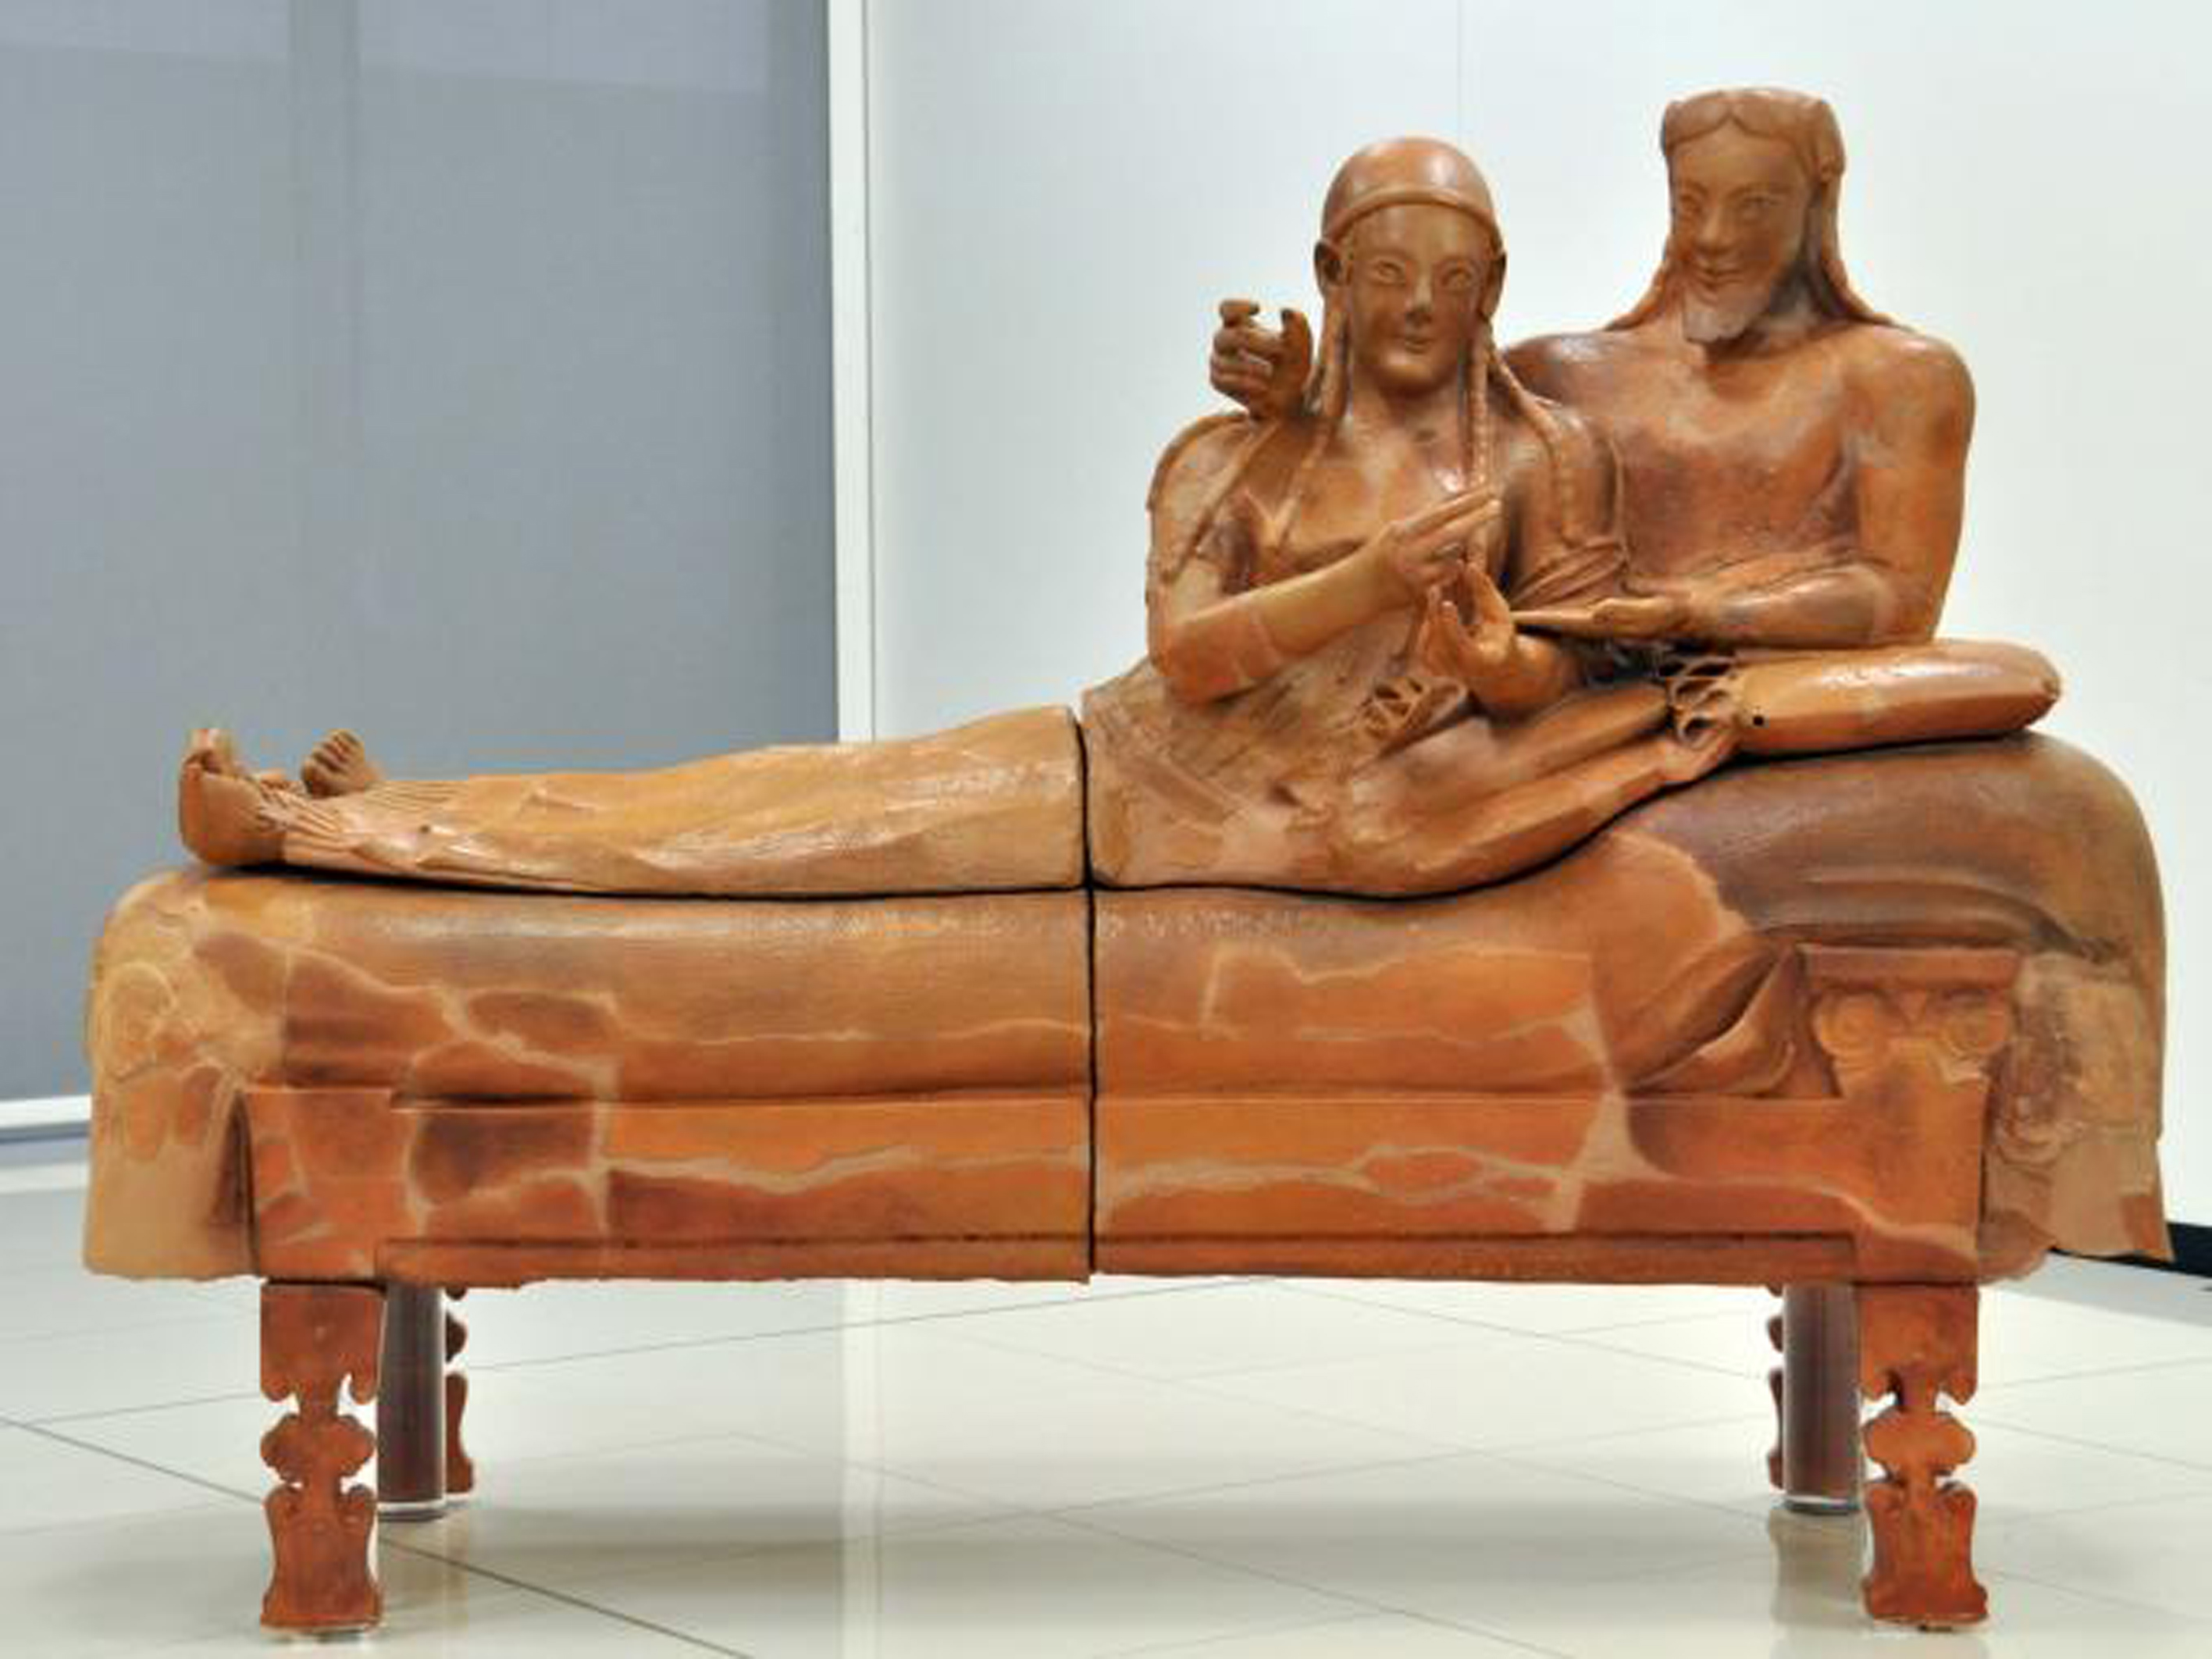
\includegraphics[width=\columnwidth]{7CloneSarcophagusoftheSpouses.jpg}
\caption{The clone of the Sarcophagus of the Spouses (scale 1:1) starting from the digital tridimensional scan of the
original Sarcophagus, Italdesign Giugiaro}
\label{fig:7}
\end{figure}


This technique would be very valid when used in the case of reproduction of mosaics and inscriptions in the mosaic.
These reproductions make for the best situation where the user can differentiate between the various levels. The
background can be made on one level, while the drawn design can be made on another upon which it is possible to write. The
use of 3D would obtain a result similar to that by the Federazione Nazionale delle Istituzioni Pro Ciechi (National
Federation of Institutions for the Blind) NPO in the Square of the Corporations of Ostia Antica. In this area, paved
with many squares of mosaics, which bear witness to the intense commercial activity of ancient Ostia, the reproduction
of Ostia’s famous lighthouse was created with different levels of elevation of a mosaic in black and white, which allow
the user not only to understand the image, but also to understand the technique of its realization. In this case,
though, the reproduction does not contain writing, because the chosen image contained no inscriptions. But nothing
prevents the use of the same technique using written entries, notwithstanding the need for an additional explanatory
panel. The disadvantage of this technique is the high cost of implementation, given that it is a reproduction created
exclusively from a specific work, and requiring a rather high level of craftsmanship since it is not merely modeled
from a metal matrix.

\begin{figure}[!hbp]
\centering
 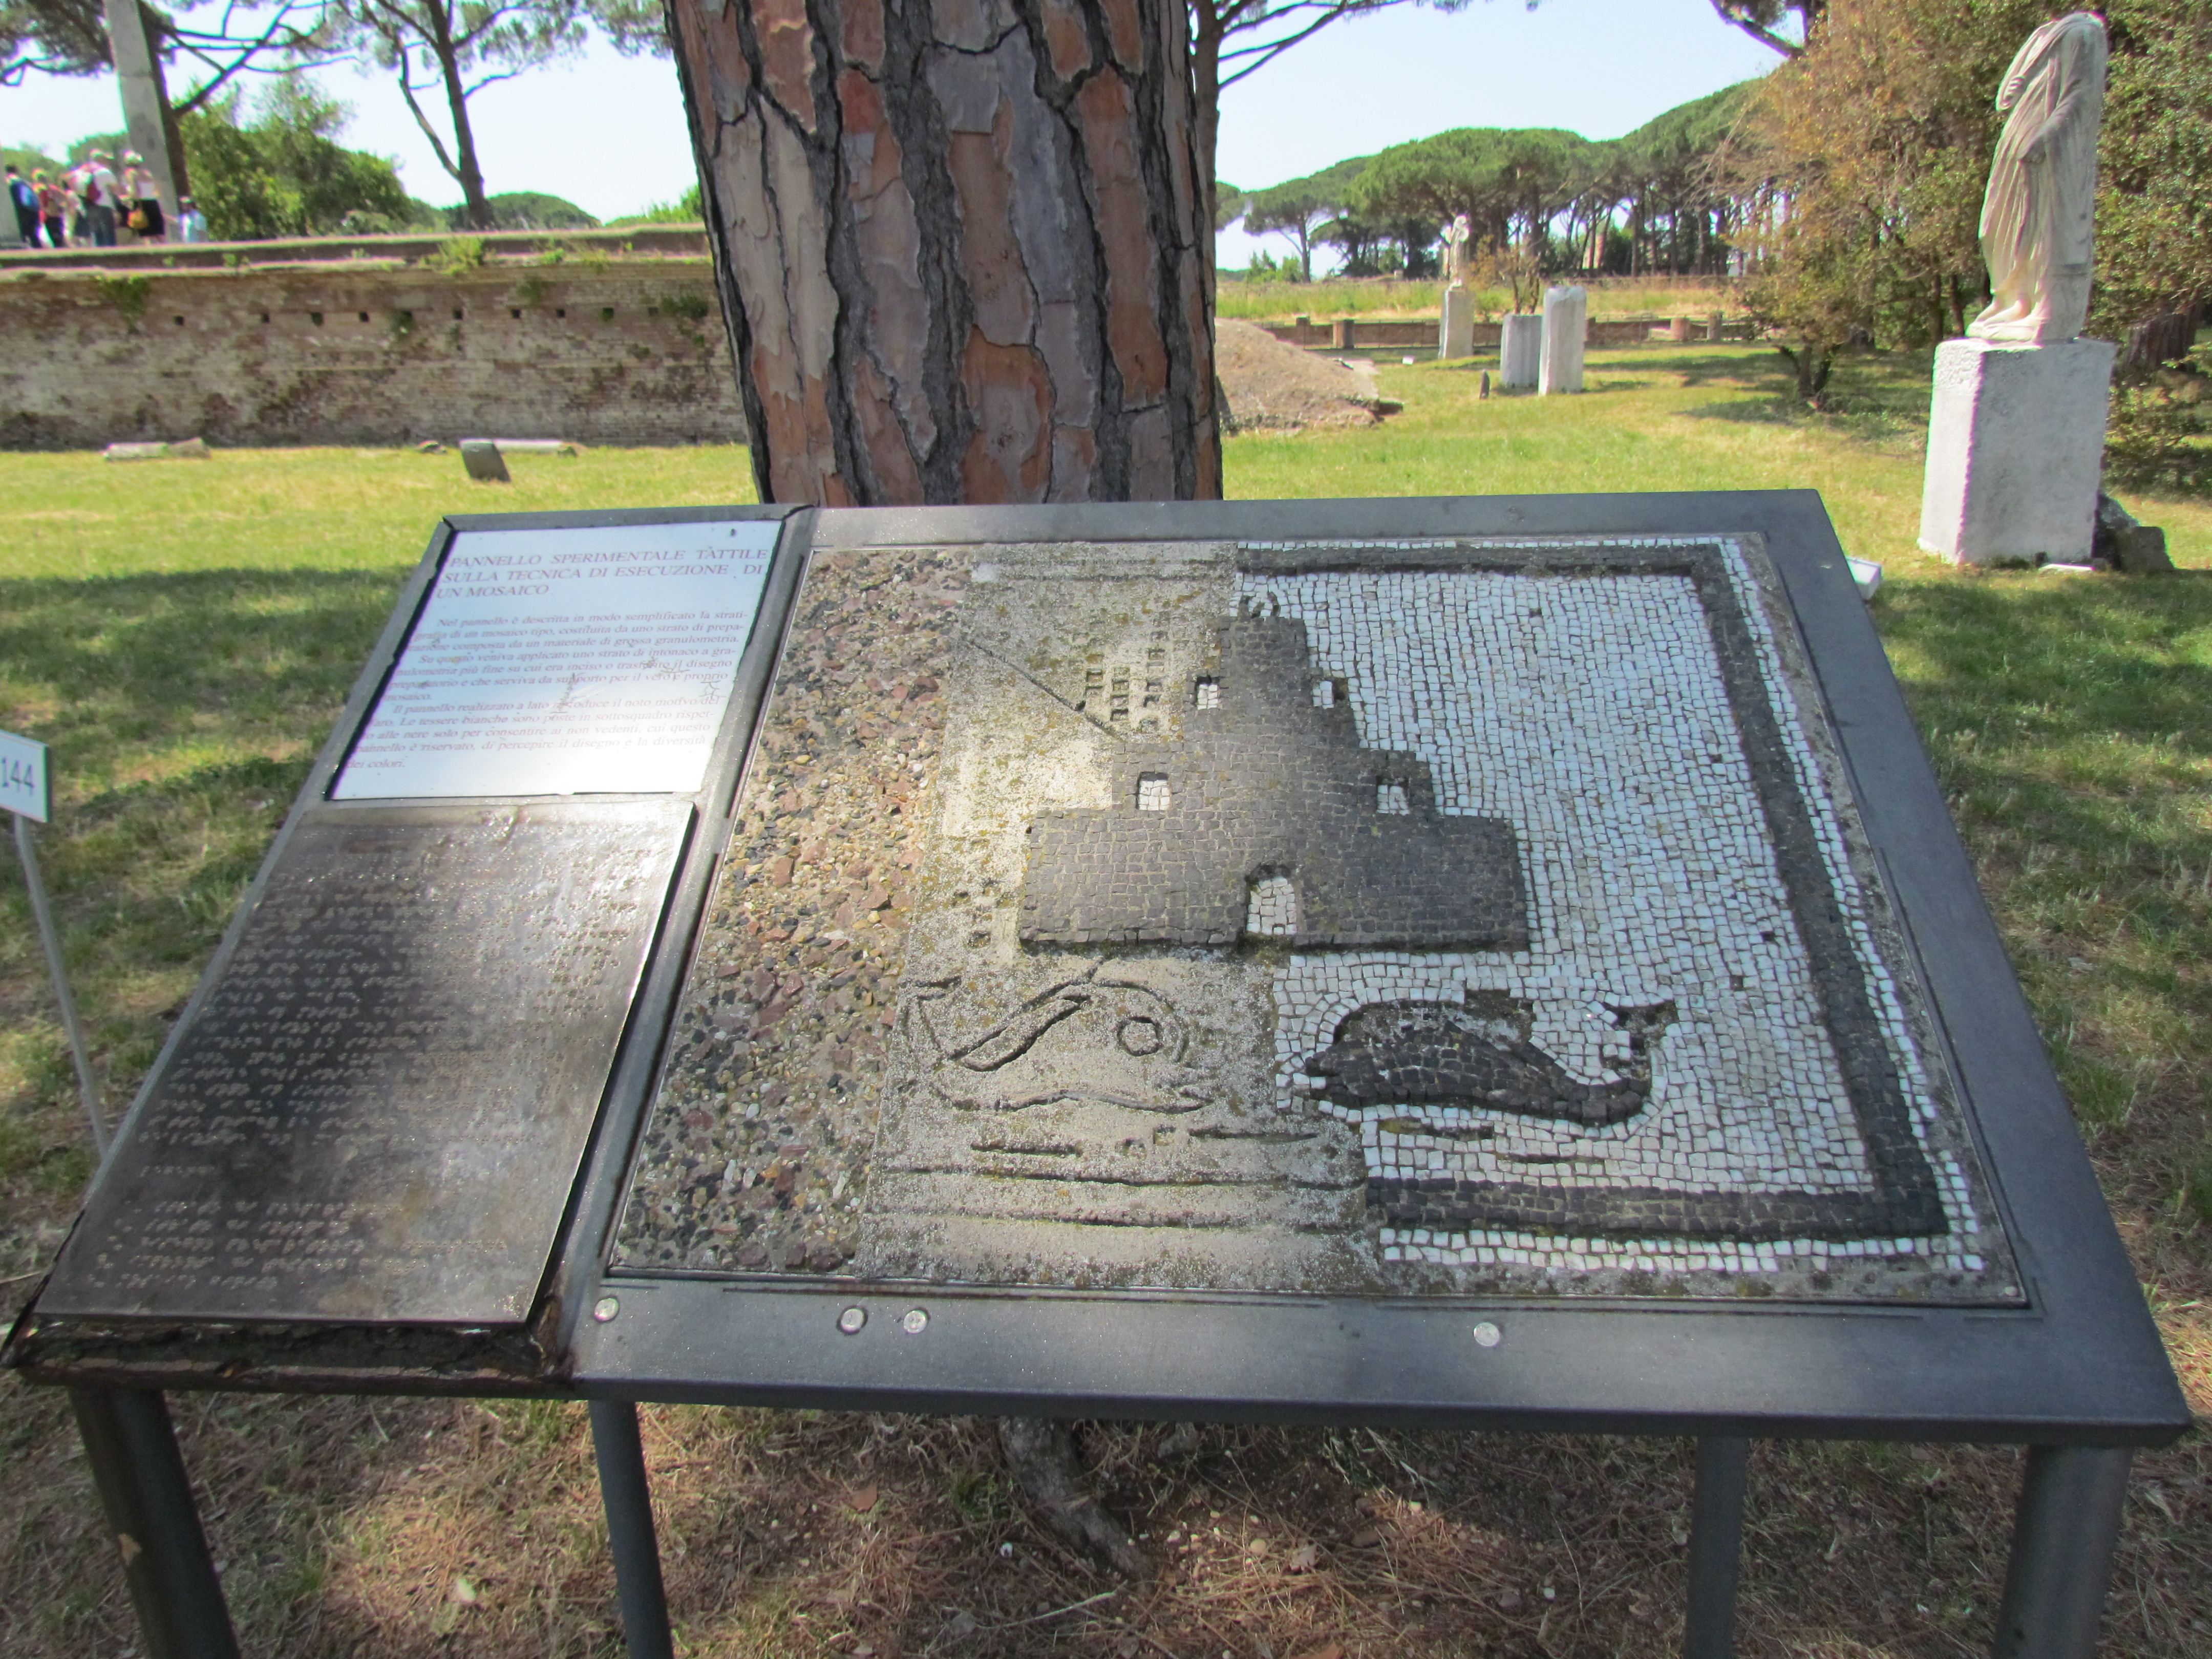
\includegraphics[width=\columnwidth]{8reproductionOstiaslighthouse.JPG}
\caption{The reproduction of the mosaic of Ostia’s lighthouse by the Federazione Nazionale delle Istituzioni Pro Ciechi NPO in the Square of the Corporations of Ostia Antica}
\label{fig:8}
\end{figure}


A thesis paper, of the Postgraduate School of Archaeological Heritage in Latin Epigraphy \citep{Licordari2015}, which
supports an exhibition project for the dissemination of Latin Epigraphy to the public, proposes 3D reproduction of two
mosaics of the stationes of that square in Ostia, with images and writing – that of the Libyan boatmen of Sabratha and
of the Carthaginian boatmen. The first, with the inscription STAT. SABRATENSIVM [CIL 14, 4549.14], is characterized by
the image of an elephant, the symbol of the Sabratha ivory trade. The second contains the inscription -NAVICVL.
KARTHAG. DE SVO [CIL 14, 4549.18] along with two ships. The paper’s original idea was based on the fact that not only
should there be brief and easy to understand inscriptions, but that the understanding could be made easier by the
presence of drawings presumably known to blind people. Certainly the case of Ostia Antica is a particularly simple one
as it involves mosaics of only two colors. A more complicated case would be a polychrome mosaic which attempts to
assimilate all the aspects of a colored painting. It is obvious that the sketched designs and writing can be configured
and presented on different levels.

\begin{figure}[!hbp]
\centering
 \includegraphics[width=\columnwidth]{9mosaicoftheLibyanboatmen.jpg}
\caption{The mosaic of the Libyan boatmen in Ostia Antica}
\label{fig:9}
\end{figure}


3D printing has the great advantage of allowing the reproduction of colors. But to be made adequately perceptible by the
visually impaired, they should have a marked color contrast.

In the thesis mentioned above was proposed the use of 3D printing for the reproduction of other artifacts containing
inscriptions. It presented the case of a portable timepiece and an Italic mirror, both objects containing images with a
few written words. The inspiration to utilize the mirror came from the creation of a computer model by the former
Superintendence of the Archaeological Heritage of Southern Etruria. Achieving the goal required the difficult
extraction from the print of a mirror with correct reproductions of the images and the script. According to the officer
in charge, it would have been enough only to deepen the furrows of the incisions in order to construct an object that
could be accessed by the blind; but this obviously does not solve the problems already analyzed. The idea in principle
is good, but modifications need to be made to the relief of the writing and the images. Given the small size of the
object in this case, provisions would need to be made for reproductions of larger scale originals in order to enlarge
the space available for the user to engage in tactile perception. It is obvious that in cases involving a different
scale from the original, it is absolutely necessary to accurately render the differences so as not to create a false
perception.

A further advantage of 3D printing is that its process is not a stranger to digital epigraphy, since its starting point
is the obtaining of a virtual model of the inscription, which is then easily printed. While the processes of
thermo-formed and Braille prints require the contacting of the respective authorities in the specialized industries or
in publishing houses, it is much easier to buy and to utilize a 3D printer in a museum, in a superintendence or in a
university. It is important to remember that whatever technique is used, it is always necessary to consult an
appropriate expert to secure the necessary guidance in the preparation of materials. It is not enough to simply take a
photo or to draw a picture and print it in 3D. The technical support of someone experienced in this field, someone who
knows the psychological and physiological characteristics of the experiential perception in the context of its tangible
modeling is absolutely necessary.

Although in the Epigraphy is a marginal aspect, it is worth mentioning the problem of material, which of course does not
solve the issues involved in 3D printing. A reproduction in resin will never give the feeling of actually touching
stone, marble or bronze material, even if treating it’s surface in a way as to give an antique effect and feeling. The
technique of reproduction is therefore very useful to facilitate experiential understanding, but only as support to the
actual experience of the original. One should of course not think that a copy can completely replace the experience of
the original object.



\begin{figure}[!hbp]
\centering
 \includegraphics[width=\columnwidth]{10italicmirror.jpg}
\caption{A mirror from Praeneste  in the National Etruscan Museum of Villa Giulia in Rome}
\label{fig:10}
\end{figure}




\section{Conclusions}
\noindent As can be seen, the studies in this field as well as the examples of works on which to experiment with seeing impaired
users are as yet few in number. We hope that this essay will lead to inspire a dialogue among the relevant experts, and
that more work will be done in the field of epigraphy to make it increasingly accessible for persons with visual
disabilities.

The use of 3D technology for the reproduction of epigraphic material is in our opinion very promising. But it requires a
substantial amount of materials to be physically touched by the blind and visually impaired, so as in this way to
increase our knowledge of how to further improve the current techniques of modeling and reproduction.

\nocite{accessibilita,Bellini2000,Cetorelli2004,Hersh2008,Jansson2003,Levi2015,Velestino2007}


\bibliographystyle{sapauth-eng}
\bibliography{../../EAGLE}

\end{document}
